\documentclass{beamer}

\title{An argumentation based solution to making schedules}
\author{Pim van der Meulen \and Ren\'e Mellema \and Xeryus Stokkel}
\date{October 24, 2016}

\usetheme{Luebeck}

\begin{document}

\frame{\titlepage}

\section{Introduction}
\begin{frame}
	\frametitle{Introduction}
	
\includegraphics[width=0.52\textwidth]{Schedule.jpg}%
	
\includegraphics[width=0.48\textwidth]{Argument.jpg}
\end{frame}

\section{State of the art}
\subsection{Syllabus Plus}
\begin{frame}
	\frametitle{Syllabus Plus}
	\begin{columns}%[c] % the "c" option specifies center vertical alignment
    \column{.4\textwidth} % column designated by a command
    \begin{itemize}
		\item Used by many colleges/universities
		\item Constraint satisfaction problem solver:
		\begin{itemize}
			\item Constraints 
			\item Rules
			\item Preferences
		\end{itemize}
	\end{itemize}
    \column{.6\textwidth}
    
\includegraphics[width=\textwidth]{SyllabusPlus.png}
    \end{columns}	
\end{frame}

\begin{frame}
\frametitle{Flow}
\center
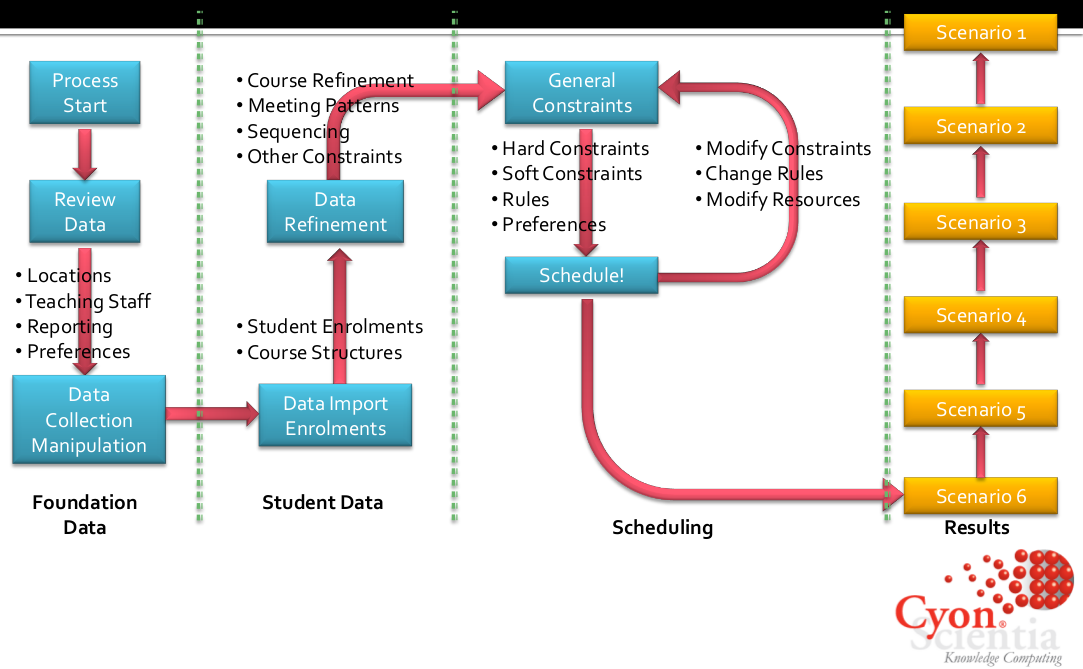
\includegraphics[width=0.9\textwidth]{SyllabusPlusFlow.png}
\end{frame}

\subsection{Kuo et al. (2011)}
\begin{frame}
\frametitle{Kuo et al. (2011)}
\begin{itemize}
\item Multi-Agent Automatic Negotiation and Argumentation for Courses Scheduling
\end{itemize}
\center
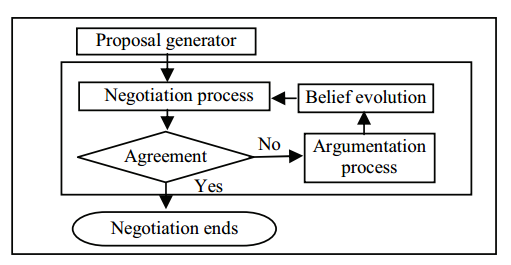
\includegraphics[width=0.9\textwidth]{Kuo1.png}
\end{frame}

\begin{frame}
\frametitle{Argumentation Phase}
\center
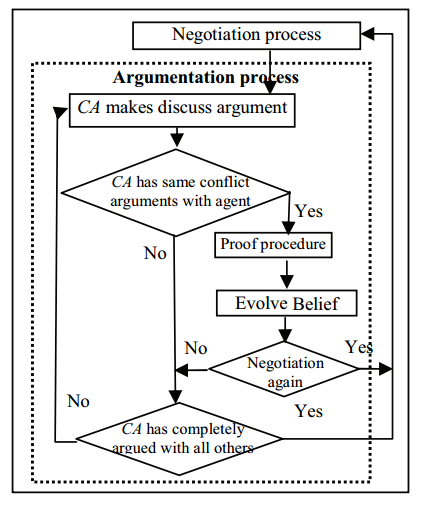
\includegraphics[width=0.5\textwidth]{Kuo2.png}
\end{frame}

\section{Our approach}
\subsection{Argumentation Framework}
\begin{frame}
    \frametitle{Argumentation Framework}
    \begin{columns}
        \column{.6\textwidth}
        \begin{itemize}
            \item Argument relations:
                \begin{itemize}
                    \item Attack
                    \item Support
                    \item Undercut
                \end{itemize}
            \item Groundedness:
                \begin{itemize}
                    \item No attacks
                    \item More support than attack
                \end{itemize}
        \end{itemize}
        \column{.4\textwidth}
        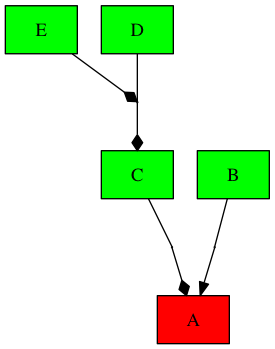
\includegraphics[width=\textwidth]{framework.png}
    \end{columns}
\end{frame}

\subsection{Scheduling}
\begin{frame}
	\frametitle{Scheduling}
        \begin{itemize}
            \item Go over all available rooms and times
            \item Agents (``Lecturers'') make claim if course fit
            \item Agents support their arguments, undercut others
            \item Continues until no new arguments are made
            \item Claim that is grounded at the end wins
        \end{itemize}
\end{frame}

\subsection{Types of arguments to use}
\begin{frame}
	\frametitle{Argument types}
	\begin{enumerate}
		\item Size argument 
		\item Beamer argument
		\item Preference argument
	\end{enumerate}
\end{frame}

\subsection{Data input}
\begin{frame}
	\frametitle{Data input}
	\center{}
	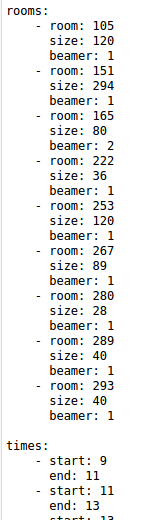
\includegraphics[width=0.2\textwidth]{Rooms.png}%
	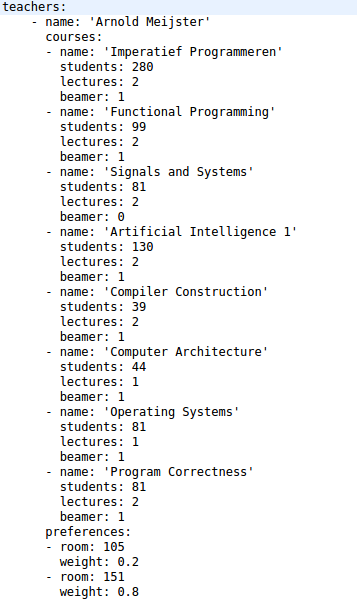
\includegraphics[width=0.365\textwidth]{Teachers.png}
\end{frame}

\section{Demo}
\begin{frame}
	\frametitle{Demo}
	Who wants to teach at this moment?
	\fontsize{6}{7.2}\selectfont
	\begin{table}
		\centering
		\caption{Friday}
		\begin{tabular}{l|r|l|l}
			Time & Room & Course & Teacher \\ \hline
			\hline
			9:00:00 & 105 & Arguing Agents & Bart Verheij\\
			& 151 & Multi Agent Systems & Rineke Verbrugge\\
			& 267 & Parallel Computing & Nicolai Petkov\\\hline
			11:00:00 & 105 & Social Complexity & Rineke Verbrugge\\
			& 267 & Signals and Systems & Arnold Meijster\\\hline
			13:00:00 & 105 & Computer Architecture & Arnold Meijster\\
			& \textbf{151} & \textbf{??} & \textbf{??}\\\hline
			15:00:00 & 105 & Formal Models of Cognition & Marieke van Vugt\\
			& 151 & Imperatief Programmeren & Arnold Meijster\\
			\end{tabular}
	\end{table}
\end{frame}

\begin{frame}[plain]
	\begin{figure}
		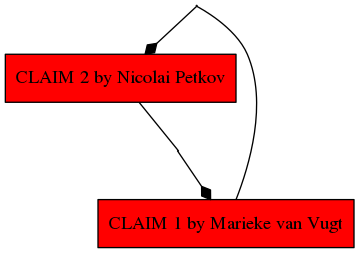
\includegraphics[keepaspectratio,width=\textwidth,height=\textheight,]{demo/claims}
	\end{figure}
\end{frame}

\begin{frame}[plain]
	\begin{figure}
		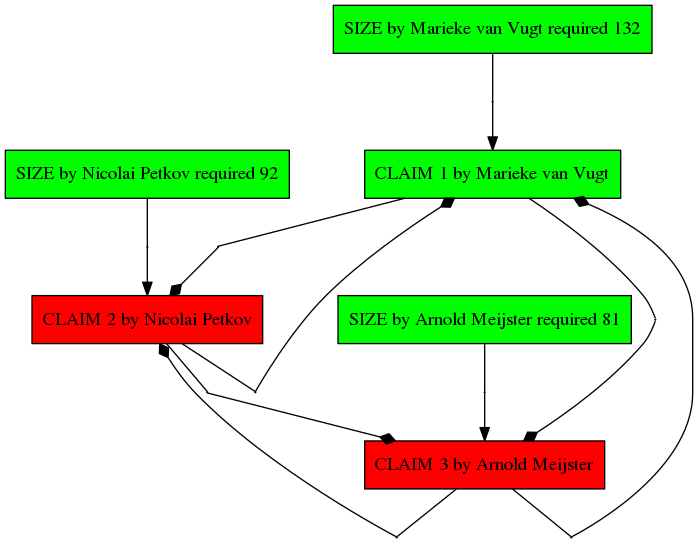
\includegraphics[keepaspectratio,width=\textwidth,height=\textheight,]{demo/0}
	\end{figure}
\end{frame}

\begin{frame}[plain]
	\begin{figure}
		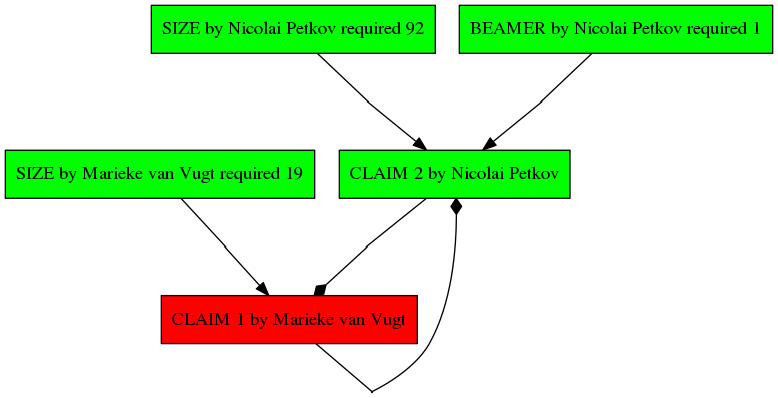
\includegraphics[keepaspectratio,width=\textwidth,height=\textheight,]{demo/1}
	\end{figure}
\end{frame}

\begin{frame}[plain]
	\begin{figure}
		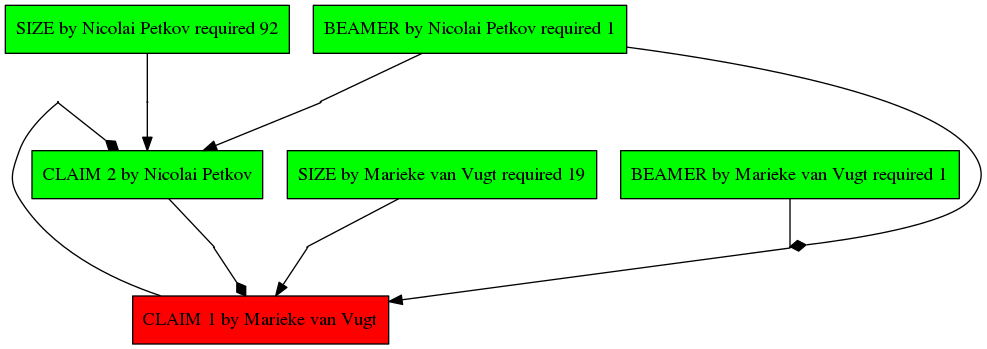
\includegraphics[keepaspectratio,width=\textwidth,height=\textheight,]{demo/2}
	\end{figure}
\end{frame}

\begin{frame}[plain]
	\begin{figure}
		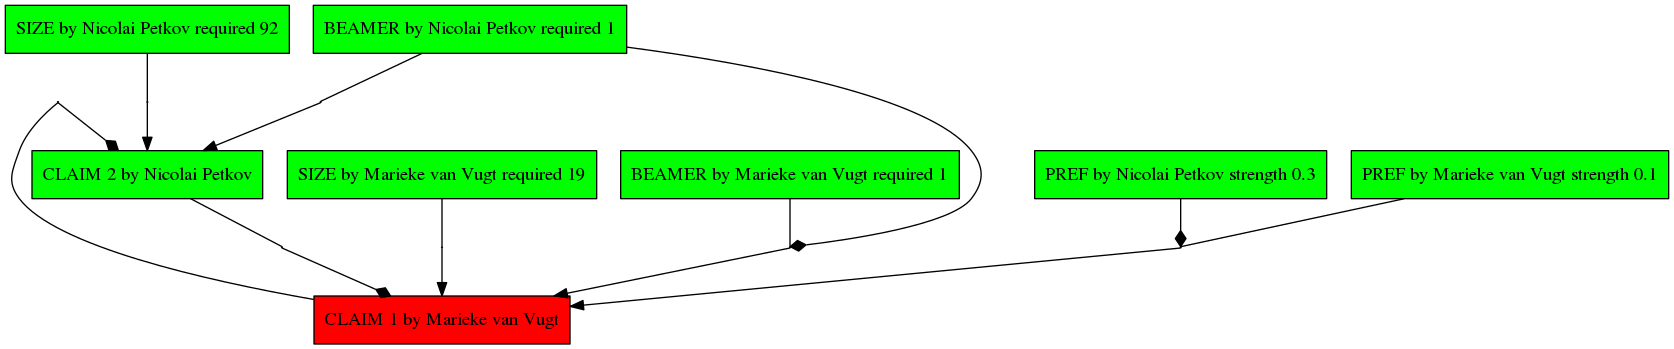
\includegraphics[keepaspectratio,width=\textwidth,height=\textheight,]{demo/3}
	\end{figure}
\end{frame}

\begin{frame}[plain]
	\begin{figure}
		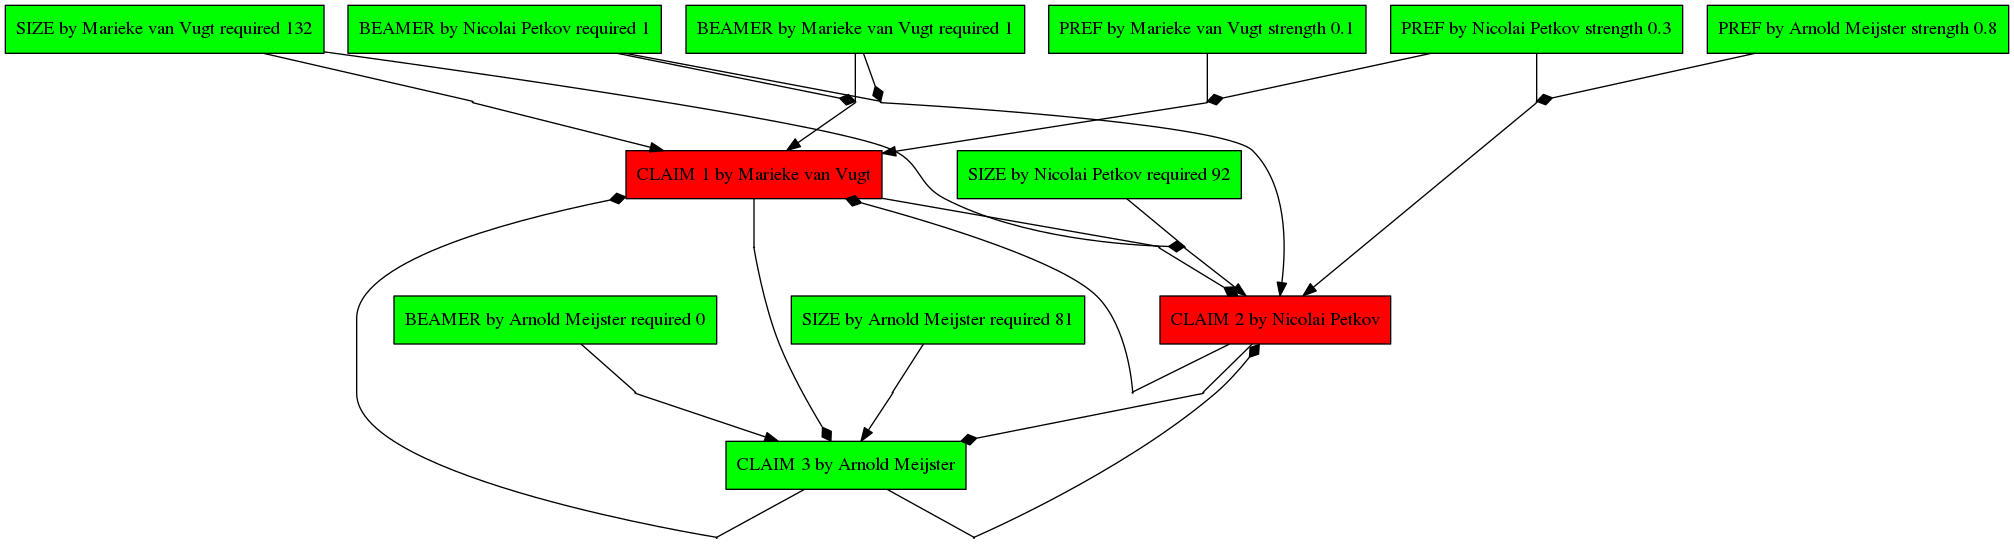
\includegraphics[keepaspectratio,width=\textwidth,height=\textheight,]{demo/4}
	\end{figure}
\end{frame}

\begin{frame}
	\frametitle{Demo}
	Finally: Nicolai Petkov will teach Introduction Intelligent Systems
	\fontsize{6}{7.2}\selectfont
	\begin{table}
		\centering
		\caption{Friday}
		\begin{tabular}{l|r|l|l}
			Time & Room & Course & Teacher \\ \hline
			\hline
			9:00:00 & 105 & Arguing Agents & Bart Verheij\\
			& 151 & Multi Agent Systems & Rineke Verbrugge\\
			& 267 & Parallel Computing & Nicolai Petkov\\\hline
			11:00:00 & 105 & Social Complexity & Rineke Verbrugge\\
			& 267 & Signals and Systems & Arnold Meijster\\\hline
			13:00:00 & 105 & Computer Architecture & Arnold Meijster\\
			& 151 & Introduction Intelligent Systems & Nicolai Petkov\\\hline
			15:00:00 & 105 & Formal Models of Cognition & Marieke van Vugt\\
			& 151 & Imperatief Programmeren & Arnold Meijster\\
			\end{tabular}
	\end{table}
\end{frame}

\section{Results}
\begin{frame}
	\frametitle{Results}
\end{frame}

\section{Relevance}
\begin{frame}
	\frametitle{Relevance}
        \begin{itemize}[<+->]
            \item Generalized for resource negotiation in MAS
            \item Extract reasons for room allocation
        \end{itemize}
\end{frame}

\frame{\frametitle{Questions?}}

\end{document}